% Options for packages loaded elsewhere
\PassOptionsToPackage{unicode}{hyperref}
\PassOptionsToPackage{hyphens}{url}
%
\documentclass[
  a4paper,
  DIV=11,
  numbers=noendperiod]{scrreport}

\usepackage{amsmath,amssymb}
\usepackage{lmodern}
\usepackage{iftex}
\ifPDFTeX
  \usepackage[T1]{fontenc}
  \usepackage[utf8]{inputenc}
  \usepackage{textcomp} % provide euro and other symbols
\else % if luatex or xetex
  \usepackage{unicode-math}
  \defaultfontfeatures{Scale=MatchLowercase}
  \defaultfontfeatures[\rmfamily]{Ligatures=TeX,Scale=1}
  \setmainfont[]{ClearSans}
\fi
% Use upquote if available, for straight quotes in verbatim environments
\IfFileExists{upquote.sty}{\usepackage{upquote}}{}
\IfFileExists{microtype.sty}{% use microtype if available
  \usepackage[]{microtype}
  \UseMicrotypeSet[protrusion]{basicmath} % disable protrusion for tt fonts
}{}
\makeatletter
\@ifundefined{KOMAClassName}{% if non-KOMA class
  \IfFileExists{parskip.sty}{%
    \usepackage{parskip}
  }{% else
    \setlength{\parindent}{0pt}
    \setlength{\parskip}{6pt plus 2pt minus 1pt}}
}{% if KOMA class
  \KOMAoptions{parskip=half}}
\makeatother
\usepackage{xcolor}
\usepackage[lmargin=2.54 cm,rmargin=2.54 cm,tmargin=2.54 cm,bmargin=2.54
cm]{geometry}
\setlength{\emergencystretch}{3em} % prevent overfull lines
\setcounter{secnumdepth}{5}
% Make \paragraph and \subparagraph free-standing
\ifx\paragraph\undefined\else
  \let\oldparagraph\paragraph
  \renewcommand{\paragraph}[1]{\oldparagraph{#1}\mbox{}}
\fi
\ifx\subparagraph\undefined\else
  \let\oldsubparagraph\subparagraph
  \renewcommand{\subparagraph}[1]{\oldsubparagraph{#1}\mbox{}}
\fi


\providecommand{\tightlist}{%
  \setlength{\itemsep}{0pt}\setlength{\parskip}{0pt}}\usepackage{longtable,booktabs,array}
\usepackage{calc} % for calculating minipage widths
% Correct order of tables after \paragraph or \subparagraph
\usepackage{etoolbox}
\makeatletter
\patchcmd\longtable{\par}{\if@noskipsec\mbox{}\fi\par}{}{}
\makeatother
% Allow footnotes in longtable head/foot
\IfFileExists{footnotehyper.sty}{\usepackage{footnotehyper}}{\usepackage{footnote}}
\makesavenoteenv{longtable}
\usepackage{graphicx}
\makeatletter
\def\maxwidth{\ifdim\Gin@nat@width>\linewidth\linewidth\else\Gin@nat@width\fi}
\def\maxheight{\ifdim\Gin@nat@height>\textheight\textheight\else\Gin@nat@height\fi}
\makeatother
% Scale images if necessary, so that they will not overflow the page
% margins by default, and it is still possible to overwrite the defaults
% using explicit options in \includegraphics[width, height, ...]{}
\setkeys{Gin}{width=\maxwidth,height=\maxheight,keepaspectratio}
% Set default figure placement to htbp
\makeatletter
\def\fps@figure{htbp}
\makeatother

\usepackage{booktabs}
\usepackage{longtable}
\usepackage{array}
\usepackage{multirow}
\usepackage{wrapfig}
\usepackage{float}
\usepackage{colortbl}
\usepackage{pdflscape}
\usepackage{tabu}
\usepackage{threeparttable}
\usepackage{threeparttablex}
\usepackage[normalem]{ulem}
\usepackage{makecell}
\usepackage{xcolor}
\KOMAoption{captions}{tableheading,figureheading}
\makeatletter
\makeatother
\makeatletter
\@ifpackageloaded{bookmark}{}{\usepackage{bookmark}}
\makeatother
\makeatletter
\@ifpackageloaded{caption}{}{\usepackage{caption}}
\AtBeginDocument{%
\ifdefined\contentsname
  \renewcommand*\contentsname{Table of contents}
\else
  \newcommand\contentsname{Table of contents}
\fi
\ifdefined\listfigurename
  \renewcommand*\listfigurename{List of Figures}
\else
  \newcommand\listfigurename{List of Figures}
\fi
\ifdefined\listtablename
  \renewcommand*\listtablename{List of Tables}
\else
  \newcommand\listtablename{List of Tables}
\fi
\ifdefined\figurename
  \renewcommand*\figurename{Figure}
\else
  \newcommand\figurename{Figure}
\fi
\ifdefined\tablename
  \renewcommand*\tablename{Table}
\else
  \newcommand\tablename{Table}
\fi
}
\@ifpackageloaded{float}{}{\usepackage{float}}
\floatstyle{ruled}
\@ifundefined{c@chapter}{\newfloat{codelisting}{h}{lop}}{\newfloat{codelisting}{h}{lop}[chapter]}
\floatname{codelisting}{Listing}
\newcommand*\listoflistings{\listof{codelisting}{List of Listings}}
\makeatother
\makeatletter
\@ifpackageloaded{caption}{}{\usepackage{caption}}
\@ifpackageloaded{subcaption}{}{\usepackage{subcaption}}
\makeatother
\makeatletter
\@ifpackageloaded{tcolorbox}{}{\usepackage[many]{tcolorbox}}
\makeatother
\makeatletter
\@ifundefined{shadecolor}{\definecolor{shadecolor}{rgb}{.97, .97, .97}}
\makeatother
\makeatletter
\makeatother
\ifLuaTeX
  \usepackage{selnolig}  % disable illegal ligatures
\fi
\IfFileExists{bookmark.sty}{\usepackage{bookmark}}{\usepackage{hyperref}}
\IfFileExists{xurl.sty}{\usepackage{xurl}}{} % add URL line breaks if available
\urlstyle{same} % disable monospaced font for URLs
\hypersetup{
  pdftitle={Analysis of Age and Gender Characteristics Among Patients with Mental Disorders},
  hidelinks,
  pdfcreator={LaTeX via pandoc}}

\title{Analysis of Age and Gender Characteristics Among Patients with
Mental Disorders}
\author{}
\date{20 September 2023}

\begin{document}
\maketitle
\ifdefined\Shaded\renewenvironment{Shaded}{\begin{tcolorbox}[frame hidden, breakable, borderline west={3pt}{0pt}{shadecolor}, enhanced, interior hidden, boxrule=0pt, sharp corners]}{\end{tcolorbox}}\fi

\renewcommand*\contentsname{Table of contents}
{
\setcounter{tocdepth}{2}
\tableofcontents
}
\bookmarksetup{startatroot}

\hypertarget{about-this-report}{%
\chapter{About this report}\label{about-this-report}}

This report is about the prevalence of mental disorders, breaking it
down by age and gender characteristics. It analyses the characteristics
of mental disorder patients and different service recipients. Data for
this report have been sourced from the Australian Bureau of Statistics
(ABS), the Australian Institute of Health and Welfare (AIHW), and the
Report on Government Services (RoGS).

In this report, the abbreviation ``MD'' is used to denote ``mental
disorder.''

\bookmarksetup{startatroot}

\hypertarget{definitions}{%
\chapter{Definitions}\label{definitions}}

\emph{Note: The phrases marked with an asterisk are explained in the
Definition section.}

\begin{itemize}
\item
  \textbf{Mental illness}: a clinically diagnosable disorder that
  significantly interferes with an individual's cognitive, emotional or
  social abilities. It covers a range of illnesses including anxiety,
  affective and substance use disorders.
\item
  \textbf{Any 12-month mental disorder}: persons who met criteria for
  diagnosis of a lifetime mental disorder (with hierarchy) and had
  sufficient symptoms of that disorder in the previous 12 months. A
  person may have more than one 12-month mental disorder.
\item
  \textbf{Lifetime mental disorders}: the number of people who met the
  diagnostic criteria for having a mental disorder at some time in their
  life. This does not imply that a person has had a mental disorder
  throughout their entire life.
\item
  \textbf{Community mental health care (CMHC)}: Community mental health
  care refers to government‑funded and operated specialised mental
  health care provided by community mental health care services and
  hospital‑based ambulatory care services, such as outpatient and day
  clinics.
\item
  \textbf{CMHC service contacts}: CMHC service contacts can be conducted
  as either individual or group sessions. Service contacts can also be
  face-to-face, via telephone, or using other forms of direct
  communication such as video link. They can be conducted in the
  presence of the patient, with a third party (such as a carer or family
  member) and/or other professional or mental health worker.
\item
  \textbf{Specialist homelessness service(s) (SHS):} Specialist
  homelessness service(s) is assistance provided by a specialist
  homelessness agency to a client aimed at responding to or preventing
  homelessness. The specialist homelessness services in scope for this
  collection include accommodation provision, assistance to sustain
  housing, mental health services, family/relationship assistance,
  disability services, drug/alcohol counselling, legal/financial
  services, immigration/cultural services, domestic/family violence
  services, other specialist services and general assistance and
  support.
\item
  \textbf{Residential mental health care (RMHC)}: Residential mental
  health care refers to residential care provided by residential mental
  health services. A residential mental health service is a specialised
  mental health service that:

  \begin{itemize}
  \item
    employs mental health trained staff on‑site
  \item
    provides rehabilitation, treatment or extended care to residents for
    whom the care is intended to be on an overnight basis and in a
    domestic‑like environment
  \item
    encourages the residents to take responsibility for their daily
    living activities.
  \end{itemize}

  These services include those that employ mental health trained staff
  on-site 24 hours per day and other services with less intensive
  staffing. However, all these services employ on‑site mental health
  trained staff for some part of the day.
\item
  \textbf{Episodes of residential care:} Episodes of residential care
  are defined as a period of care between the start of residential care
  (either through the formal start of the residential stay or the start
  of a new reference period (that is, 1 July)) and the end of
  residential care (either through the formal end of residential care,
  commencement of leave intended to be greater than 7 days, or the end
  of the reference period (that is, 30 June)). An individual can have
  one or more episodes of care during the reference period.
\item
  \textbf{Psychosocial disability:} Psychosocial disability describes a
  disability that comes from a mental health condition. Not everyone who
  has a mental health condition will have a psychosocial disability.
  Examples of some psychosocial disabilities include Schizophrenia and
  Schizoaffective disorder, Anxiety disorders, Obsessive compulsive
  disorder, Post-traumatic stress disorder, Agoraphobia and Social
  phobia or Mood disorders, such as Depression and Bipolar.
\item
  \textbf{Primary disability}: A primary disabilityis~the disability
  that causes the most difficulties in everyday life. Many people have
  multiple disabilities or other comorbid conditions that do not impair
  the person to the same extent as their primary disability. These are
  referred to as secondary disabilities.
\end{itemize}

\bookmarksetup{startatroot}

\hypertarget{prevalence-of-mental-disorders-among-adults}{%
\chapter{Prevalence of mental disorders among
adults}\label{prevalence-of-mental-disorders-among-adults}}

\hypertarget{about-the-data}{%
\section{About the data}\label{about-the-data}}

The 2020-21 National Study of Mental Health and Wellbeing (NSMHW)
measures the prevalence of mental disorders among Australians aged 16-85
years using the World Health Organization Composite International
Diagnostic Interview.

Respondents were asked about their experiences and symptoms of mental
ill-health throughout their lifetime, from which two key measures are
analysed:

\begin{itemize}
\item
  \textbf{lifetime mental disorders}, which refers to the number of
  people who met the diagnostic criteria for having a mental disorder at
  some time in their life. This does not imply that a person has had a
  mental disorder throughout their entire life
\item
  \textbf{12-month mental disorders}, which refers to the number of
  people who met the diagnostic criteria for having a mental disorder at
  some time in their life and had sufficient symptoms of that disorder
  in the 12 months prior to the survey.
\end{itemize}

Three groups of mental disorders are assessed---Anxiety, Affective and
Substance Use disorders---based on definitions and criteria of the World
Health Organization International Classification of Diseases, Tenth
Revision.

The data used for this section came from two sources:

\begin{enumerate}
\def\labelenumi{\arabic{enumi}.}
\item
  \href{https://www.pc.gov.au/ongoing/report-on-government-services/2023/health/services-for-mental-health}{Report
  on Government Services 2023}
\item
  \href{https://www.abs.gov.au/statistics/health/mental-health/national-study-mental-health-and-wellbeing/latest-release\#prevalence-of-mental-disorders}{National
  Study of Mental Health and Wellbeing}
\end{enumerate}

\emph{Note: Due to COVID-related difficulties with in-person data
collection during 2021, the National Study of Mental Health and
Wellbeing (NSMHW) was conducted in two parts from 2020 to 2022. As a
result, only national totals are available for reporting in 2023. These
data \textbf{should not be compared to the 2007 survey} due to a smaller
sample size in 2020-2021. (State and territory data are expected to be
available for the 2024 Report.)}

\hypertarget{mental-health-status}{%
\section{Mental Health Status}\label{mental-health-status}}

\hypertarget{by-sex}{%
\subsection{By Sex}\label{by-sex}}

\begin{figure}

\caption{\label{fig-mhss}Mental Health Status by Sex, 2007 and 2020-21}

{\centering 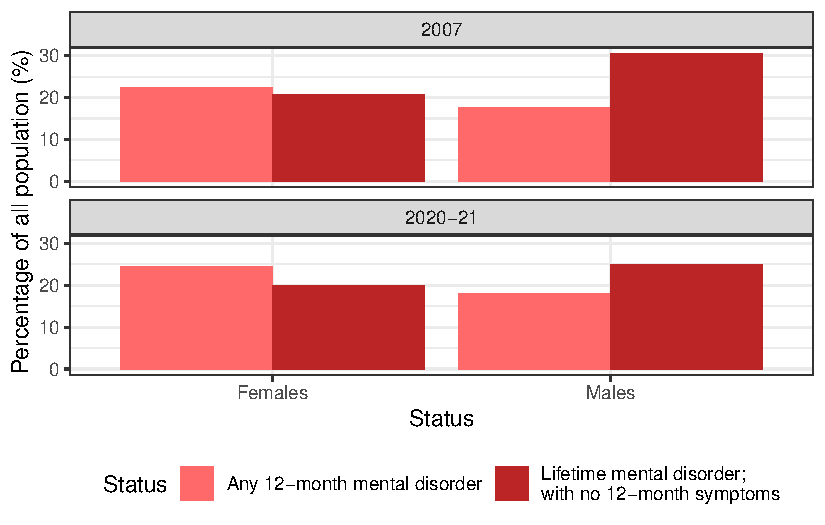
\includegraphics{./chap1-prevalence-of-md_files/figure-pdf/fig-mhss-1.pdf}

}

\end{figure}

\emph{Note: According to AIHW, 2007 and 2020-21 have different sample
sizes, so be cautious when comparing.}

\hypertarget{by-age-group}{%
\subsection{By Age Group}\label{by-age-group}}

\begin{figure}

\caption{\label{fig-mhsag}Mental Health Status by Age Group, 2007 and
2020-21}

{\centering 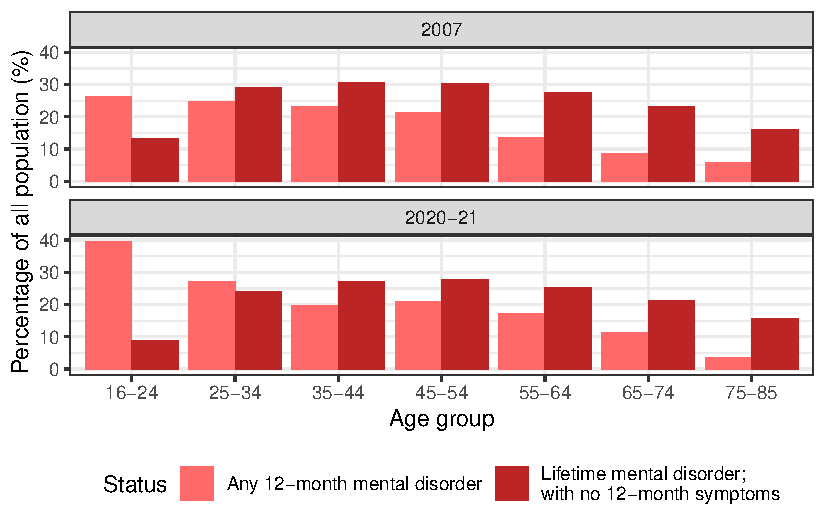
\includegraphics{./chap1-prevalence-of-md_files/figure-pdf/fig-mhsag-1.pdf}

}

\end{figure}

\emph{Note: According to AIHW, 2007 and 2020-21 have different sample
sizes, so be cautious when comparing.}

\hypertarget{summary}{%
\subsection{Summary}\label{summary}}

\begin{itemize}
\item
  In both 2007 and 2020-21, a higher proportion of females reported
  experiencing symptoms of mental disorders in the 12 months leading up
  to the survey. In contrast, a more significant percentage of males
  reported lifetime mental disorders but did not exhibit symptoms in the
  12 months prior to the survey.
\item
  In 2020-21, nearly 40\% of individuals aged 16-24 reported
  experiencing mental disorders in the 12 months prior to the survey.
  This prevalence declined with increasing age.
\item
  For those aged 25-74, between 20\% and 30\% reported having lifetime
  mental disorders without symptoms in the past 12 months. For the age
  groups 16-24 and 75-85, the figures stood at approximately 10\% and
  15\%, respectively.
\end{itemize}

\hypertarget{month-mental-disorder-categories}{%
\section{12-Month Mental Disorder
Categories}\label{month-mental-disorder-categories}}

\hypertarget{by-sex-1}{%
\subsection{By Sex}\label{by-sex-1}}

\begin{figure}

\caption{\label{fig-12s}Mental Disorder Categories by Sex, 2007 and
2020-21}

{\centering 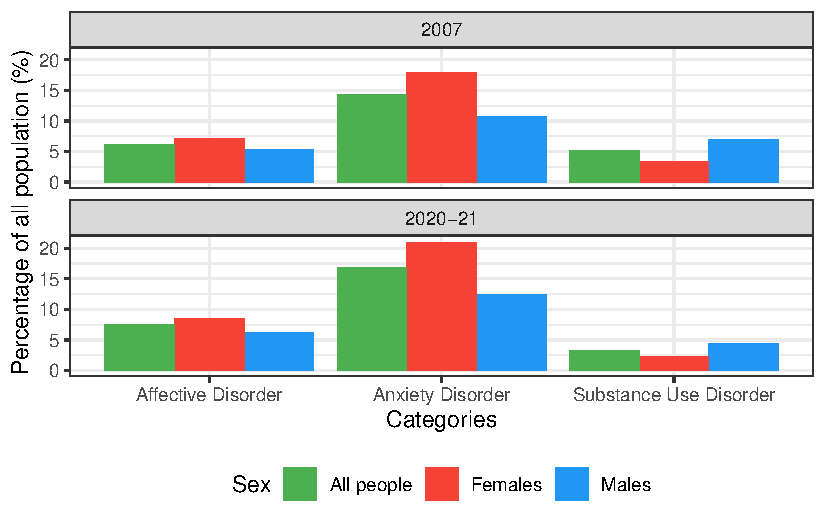
\includegraphics{./chap1-prevalence-of-md_files/figure-pdf/fig-12s-1.pdf}

}

\end{figure}

\emph{Note: According to AIHW, 2007 and 2020-21 have different sample
sizes, so be cautious when comparing.}

\hypertarget{by-age-group-1}{%
\subsection{By Age Group}\label{by-age-group-1}}

\begin{figure}

\caption{\label{fig-12a}Mental Disorder Categories by Age Group, 2007
and 2020-21}

{\centering 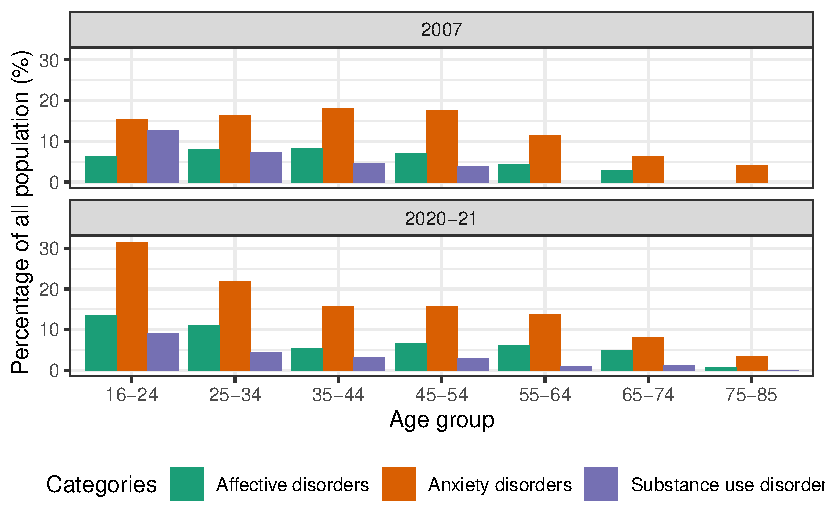
\includegraphics{./chap1-prevalence-of-md_files/figure-pdf/fig-12a-1.pdf}

}

\end{figure}

\emph{Note: According to AIHW, 2007 and 2020-21 have different sample
sizes, so be cautious when comparing.}

\hypertarget{subcategories}{%
\subsection{Subcategories}\label{subcategories}}

\hypertarget{tbl-sub}{}
\begin{table}
\caption{\label{tbl-sub}Prevalence of 12-Month Mental Disorders by Subcategory for 2020-21 and
2007 }\tabularnewline

\centering
\begin{tabular}[t]{l|>{}r|>{}r|r|>{}r|>{}r|r}
\hline
\multicolumn{1}{c|}{\textbf{ }} & \multicolumn{3}{c|}{\textbf{2020-21}} & \multicolumn{3}{c}{\textbf{2007}} \\
\cline{2-4} \cline{5-7}
\textbf{Disorder Types} & \textbf{Male(\%)} & \textbf{Female(\%)} & \textbf{All(\%)} & \textbf{Male(\%)} & \textbf{Female(\%)} & \textbf{All(\%)}\\
\hline
\multicolumn{7}{l}{\textbf{Anxiety disorders}}\\
\hline
\hspace{1em}Panic disorder & \textcolor[HTML]{2196F3}{2.3} & \textcolor[HTML]{F44336}{5.0} & 3.7 & \textcolor[HTML]{2196F3}{2.3} & \textcolor[HTML]{F44336}{2.8} & 2.6\\
\hline
\hspace{1em}Agoraphobia & \textcolor[HTML]{2196F3}{2.6} & \textcolor[HTML]{F44336}{6.7} & 4.6 & \textcolor[HTML]{2196F3}{2.1} & \textcolor[HTML]{F44336}{3.5} & 2.8\\
\hline
\hspace{1em}Social phobia & \textcolor[HTML]{2196F3}{4.3} & \textcolor[HTML]{F44336}{9.8} & 7.0 & \textcolor[HTML]{2196F3}{3.8} & \textcolor[HTML]{F44336}{5.7} & 4.7\\
\hline
\hspace{1em}Generalised anxiety disorder & \textcolor[HTML]{2196F3}{3.0} & \textcolor[HTML]{F44336}{4.7} & 3.8 & \textcolor[HTML]{2196F3}{2.0} & \textcolor[HTML]{F44336}{3.5} & 2.7\\
\hline
\hspace{1em}Obsessive compulsive disorder & \textcolor[HTML]{2196F3}{2.5} & \textcolor[HTML]{F44336}{3.8} & 3.1 & \textcolor[HTML]{2196F3}{1.6} & \textcolor[HTML]{F44336}{2.2} & 1.9\\
\hline
\hspace{1em}Post traumatic stress disorder & \textcolor[HTML]{2196F3}{3.6} & \textcolor[HTML]{F44336}{7.6} & 5.7 & \textcolor[HTML]{2196F3}{4.6} & \textcolor[HTML]{F44336}{8.3} & 6.4\\
\hline
\multicolumn{7}{l}{\textbf{Affective disorders}}\\
\hline
\hspace{1em}Depressive episode & \textcolor[HTML]{2196F3}{3.8} & \textcolor[HTML]{F44336}{5.3} & 4.6 & \textcolor[HTML]{2196F3}{3.1} & \textcolor[HTML]{F44336}{5.1} & 4.1\\
\hline
\hspace{1em}Dysthymia & \textcolor[HTML]{2196F3}{1.1} & \textcolor[HTML]{F44336}{2.1} & 1.7 & \textcolor[HTML]{2196F3}{1.0} & \textcolor[HTML]{F44336}{1.5} & 1.3\\
\hline
\hspace{1em}Bipolar affective disorder & \textcolor[HTML]{2196F3}{1.9} & \textcolor[HTML]{F44336}{2.4} & 2.2 & \textcolor[HTML]{2196F3}{1.8} & \textcolor[HTML]{F44336}{1.7} & 1.8\\
\hline
\multicolumn{7}{l}{\textbf{Substance use disorders}}\\
\hline
\hspace{1em}Alcohol harmful use & \textcolor[HTML]{2196F3}{2.2} & \textcolor[HTML]{F44336}{0.9} & 1.6 & \textcolor[HTML]{2196F3}{3.8} & \textcolor[HTML]{F44336}{2.1} & 2.9\\
\hline
\hspace{1em}Alcohol dependence & \textcolor[HTML]{2196F3}{1.1} & \textcolor[HTML]{F44336}{0.6} & 0.9 & \textcolor[HTML]{2196F3}{2.2} & \textcolor[HTML]{F44336}{0.7} & 1.4\\
\hline
\hspace{1em}Drug use disorders & \textcolor[HTML]{2196F3}{1.3} & \textcolor[HTML]{F44336}{0.6} & 1.0 & \textcolor[HTML]{2196F3}{2.1} & \textcolor[HTML]{F44336}{0.8} & 1.4\\
\hline
\end{tabular}
\end{table}

\emph{Note: According to AIHW, 2007 and 2020-21 have different sample
sizes, so be cautious when comparing.}

\hypertarget{summary-1}{%
\subsection{Summary}\label{summary-1}}

\begin{itemize}
\item
  In 2007, the prevalence of Affective disorders was consistent for
  people aged 16-74, while in 2020-21, it is more common among young
  individuals.
\item
  The prevalence of both Anxiety disorders and Substance use disorders
  in both 2007 and 2020-21 generally showed a decreasing trend with
  increasing ages.
\item
  The prevalence of Anxiety Disorder is twice as high as the other two.
  Additionally, the prevalence among females is nearly double that among
  males, especially in Agoraphobia, Social phobia, and Post-traumatic
  stress disorder.
\item
  Males had almost twice the rate of Substance Use disorder than
  females, especially in Alcohol harmful use.
\end{itemize}

\hypertarget{month-mental-health-disorder-characteristics}{%
\section{12-Month Mental Health Disorder
Characteristics}\label{month-mental-health-disorder-characteristics}}

\emph{Note:}

\begin{itemize}
\item
  \emph{Some of the prevalence number data have a relatively high
  standard error and should be used with caution.}
\item
  \emph{Percentage has a high margin of error and should be used with
  caution.}
\item
  \emph{The data have been randomly adjusted to avoid the release of
  confidential data. Discrepancies may occur between sums of the
  component items and totals.}
\end{itemize}

\hypertarget{by-age-group-generation}{%
\subsection{By Age Group (Generation)}\label{by-age-group-generation}}

\begin{figure}

\caption{\label{fig-12ag}EST. Prevalence Number and Percentage by
Generation, 2020--21}

{\centering 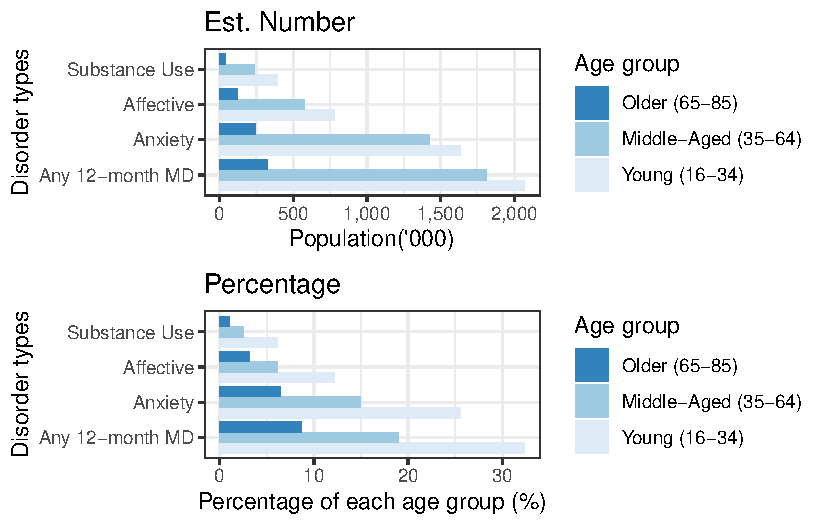
\includegraphics{./chap1-prevalence-of-md_files/figure-pdf/fig-12ag-1.pdf}

}

\end{figure}

\emph{Note: Percentages have been randomly adjusted to avoid the release
of confidential data. The percentages \textbf{do not sum to 100\%}.}

\hypertarget{by-age-group-decadal}{%
\subsection{By Age Group (Decadal)}\label{by-age-group-decadal}}

\begin{figure}

\caption{\label{fig-12ad}EST. Prevalence Number and Percentage by
Decadal Age Group, 2020--21}

{\centering 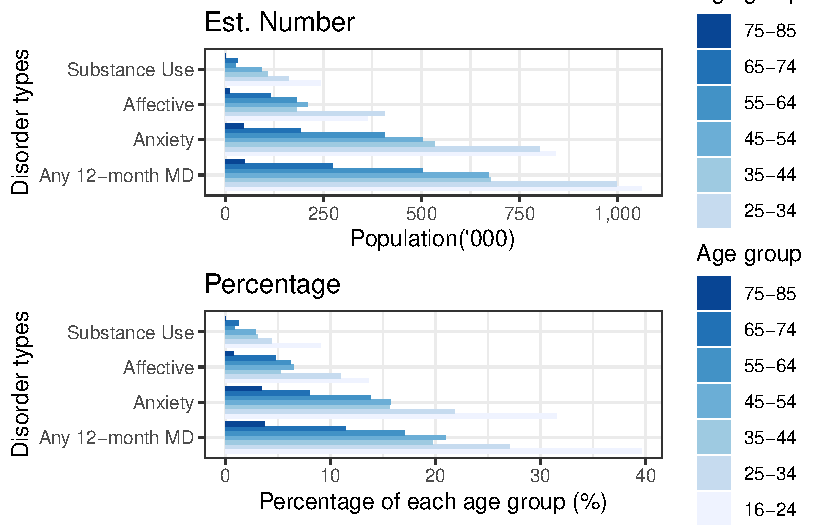
\includegraphics{./chap1-prevalence-of-md_files/figure-pdf/fig-12ad-1.pdf}

}

\end{figure}

\emph{Note: Percentages have been randomly adjusted to avoid the release
of confidential data. The percentages \textbf{do not sum to 100\%}.}

\hypertarget{by-sex-2}{%
\subsection{By Sex}\label{by-sex-2}}

\begin{figure}

\caption{\label{fig-12as}EST. Prevalence Number and Percentage by Sex,
2020--21}

{\centering 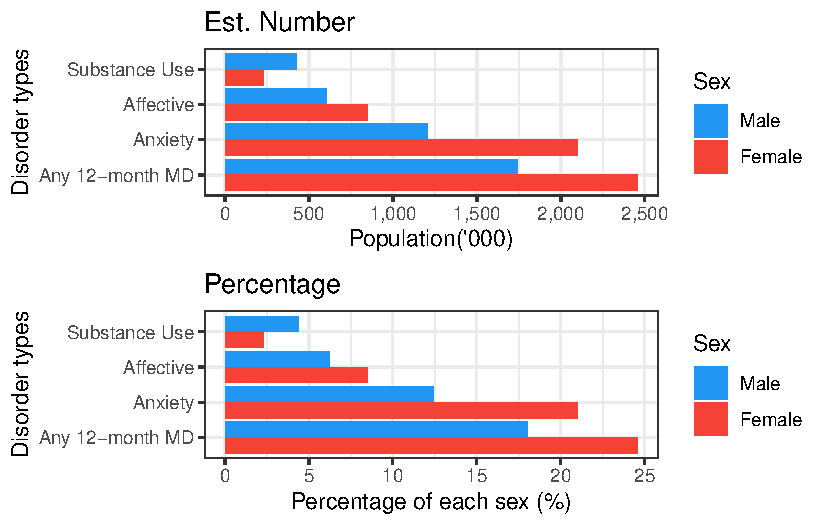
\includegraphics{./chap1-prevalence-of-md_files/figure-pdf/fig-12as-1.pdf}

}

\end{figure}

\emph{Note: Percentages have been randomly adjusted to avoid the release
of confidential data. The percentages \textbf{do not sum to 100\%}.}

\hypertarget{by-generation-and-sex}{%
\subsection{By Generation and Sex}\label{by-generation-and-sex}}

\begin{figure}

\caption{\label{fig-12gsn}EST. Prevalence Number by Generation and Sex,
2020--21}

{\centering 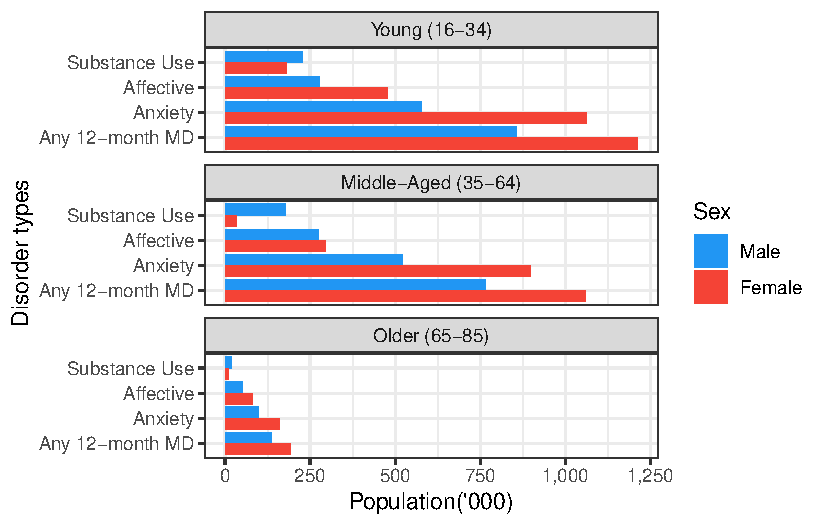
\includegraphics{./chap1-prevalence-of-md_files/figure-pdf/fig-12gsn-1.pdf}

}

\end{figure}

\begin{figure}

\caption{\label{fig-12gsp}Prevalence Percentage by Generation and Sex,
2020--21}

{\centering 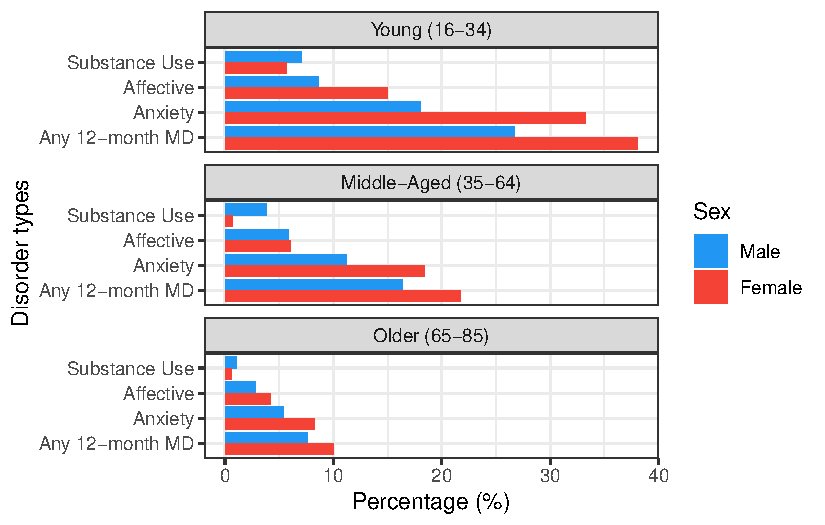
\includegraphics{./chap1-prevalence-of-md_files/figure-pdf/fig-12gsp-1.pdf}

}

\end{figure}

\emph{Note: Percentages have been randomly adjusted to avoid the release
of confidential data. The percentages \textbf{do not sum to 100\%}.}

\hypertarget{by-decadal-age-group-and-sex}{%
\subsection{By Decadal Age Group and
Sex}\label{by-decadal-age-group-and-sex}}

\begin{figure}

\caption{\label{fig-12dgn}EST. Prevalence Number by Decadal Age Group
and Sex, 2020--21}

{\centering 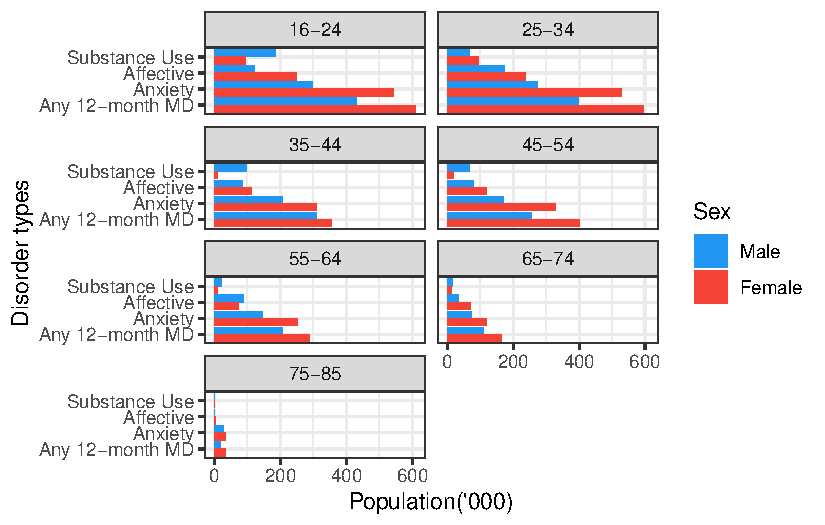
\includegraphics{./chap1-prevalence-of-md_files/figure-pdf/fig-12dgn-1.pdf}

}

\end{figure}

\begin{figure}

\caption{\label{fig-12dgp}Prevalence Percentage by Decadal Age Group and
Sex, 2020--21}

{\centering 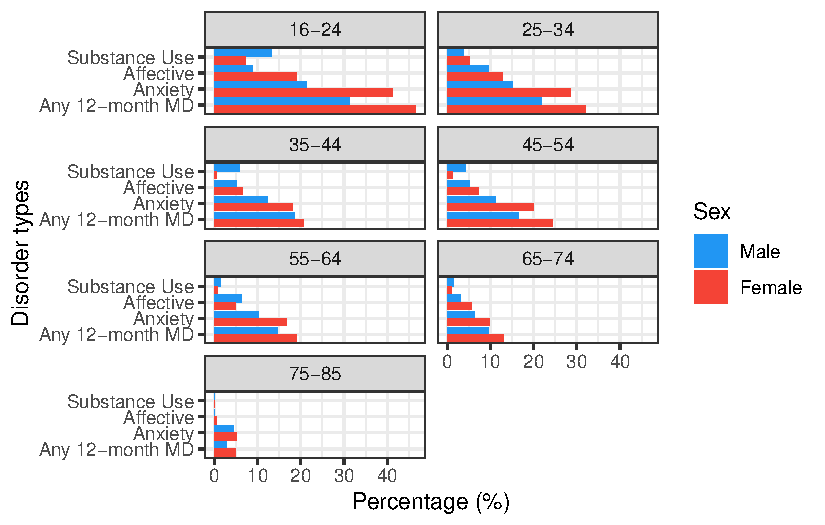
\includegraphics{./chap1-prevalence-of-md_files/figure-pdf/fig-12dgp-1.pdf}

}

\end{figure}

\emph{Note: Percentages have been randomly adjusted to avoid the release
of confidential data. The percentages \textbf{do not sum to 100\%}.}

\hypertarget{summary-2}{%
\subsection{Summary}\label{summary-2}}

\begin{itemize}
\item
  The prevalence of 12-month mental disorders is highest among young
  individuals, particularly those aged 16-24, and generally decreases
  with age.
\item
  Females consistently show a higher prevalence than males across all
  age groups.
\item
  Except for the age group 25-34, males have higher Substance Use
  Disorders than females, with a particularly noticeable high prevalence
  in the 16-24 and 35-54 age groups.
\item
  Females exhibit a remarkably higher prevalence of Anxiety Disorders
  across all age groups.
\item
  The prevalence of Affective Disorders is generally higher among
  females than males across all age groups, except for 55-64.
\end{itemize}

\bookmarksetup{startatroot}

\hypertarget{community-mental-health-care-cmhc-service}{%
\chapter{Community Mental Health Care (CMHC)
Service}\label{community-mental-health-care-cmhc-service}}

\hypertarget{about-the-data-1}{%
\section{About the Data}\label{about-the-data-1}}

Mental illness is often treated in community and hospital-based
outpatient care services provided by state and territory governments.
Collectively, these services are referred to as \textbf{community mental
health care (CMHC)} services.

The data used for this section came from
\href{https://www.aihw.gov.au/mental-health/topic-areas/community-services\#data}{Australian
Institute of Health and Welfare (AIHW)}.

\hypertarget{cmhc-patients}{%
\section{CMHC Patients}\label{cmhc-patients}}

\hypertarget{by-age-group-2}{%
\subsection{By Age Group}\label{by-age-group-2}}

\begin{figure}

\caption{\label{fig-cmhc-a}CMHC Patients by Age Group, 2020-21}

{\centering 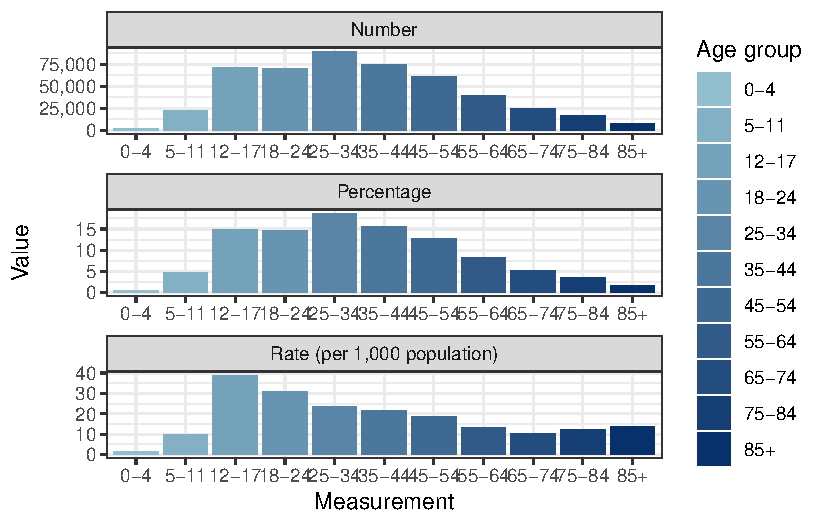
\includegraphics{./chap2-cmhc_files/figure-pdf/fig-cmhc-a-1.pdf}

}

\end{figure}

\emph{Note: Rate stands for the number of patients receiving services
per 1,000 population.}

\hypertarget{by-age-group-and-states-or-territories}{%
\subsection{By Age Group and States or
Territories}\label{by-age-group-and-states-or-territories}}

\begin{figure}

\caption{\label{fig-cmhc-asn}Number of CMHC Patients by Age Group and
States or Territories, 2020--21}

{\centering 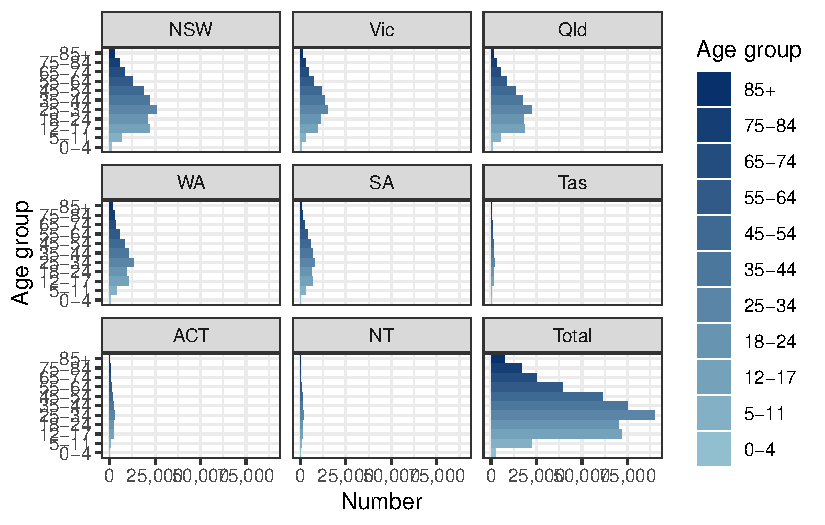
\includegraphics{./chap2-cmhc_files/figure-pdf/fig-cmhc-asn-1.pdf}

}

\end{figure}

\begin{figure}

\caption{\label{fig-cmhc-asp}Percentage of CMHC Patients by Age Group
and States or Territories, 2020--21}

{\centering 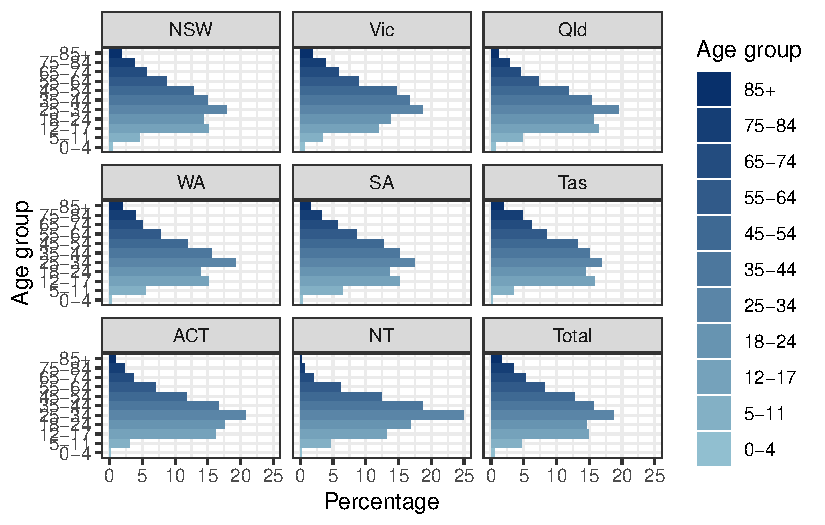
\includegraphics{./chap2-cmhc_files/figure-pdf/fig-cmhc-asp-1.pdf}

}

\end{figure}

\begin{figure}

\caption{\label{fig-cmhc-asr}Rate (Per 1,000 Population) of CMHC
Patients by Age Group and States or Territories, 2020--21}

{\centering 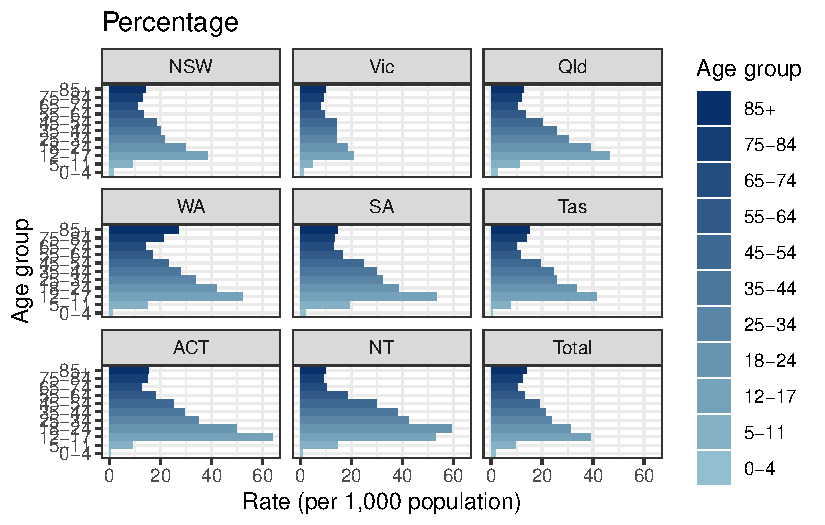
\includegraphics{./chap2-cmhc_files/figure-pdf/fig-cmhc-asr-1.pdf}

}

\end{figure}

\emph{Note: Rate stands for the number of patients receiving services
per 1,000 population.}

\hypertarget{by-sex-3}{%
\subsection{By Sex}\label{by-sex-3}}

\begin{figure}

\caption{\label{fig-cmhc-s}CMHC Patients by Sex, 2020-21}

{\centering 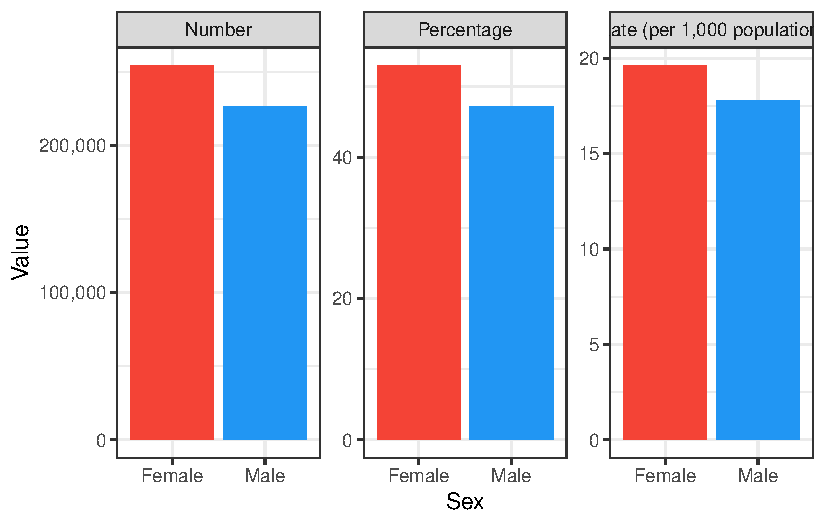
\includegraphics{./chap2-cmhc_files/figure-pdf/fig-cmhc-s-1.pdf}

}

\end{figure}

\hypertarget{by-sex-and-states-or-territories}{%
\subsection{By Sex and States or
Territories}\label{by-sex-and-states-or-territories}}

\begin{figure}

\caption{\label{fig-cmhc-ss}The Value Difference of Female and Male CMHC
Patients, 2020--21}

{\centering 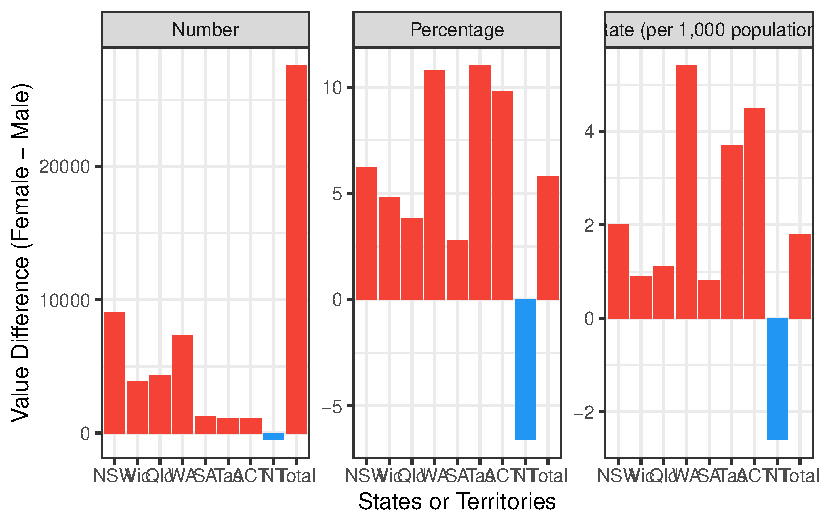
\includegraphics{./chap2-cmhc_files/figure-pdf/fig-cmhc-ss-1.pdf}

}

\end{figure}

\emph{Note: Rate stands for the number of patients receiving services
per 1,000 population.}

\hypertarget{summary-3}{%
\subsection{Summary}\label{summary-3}}

Patients rate:

\begin{itemize}
\item
  Teenagers aged 12-17 have the highest patient rates across all age
  groups.
\item
  Patient rates generally decrease with age but show an uptick for
  individuals over 75, especially in WA and Tas.
\item
  Vic has the lowest overall patient rate and shows minimal variation
  across age groups.
\item
  Females have higher patient rates than males, with exceptions in NT
  and significant trends observed in WA, ACT, and Tas.
\end{itemize}

Patient characteristics:

\begin{itemize}
\item
  The age distribution of patients exhibits a bell-shaped, right-skewed
  curve, with the peak in the 25-34 age group.
\item
  Significantly higher percentages and numbers of patients are aged
  12-17 in NSW, Qld, WA, SA, and Tas.
\item
  Except in NT, female patients outnumber male patients across all
  states. The highest numbers of female patients are found in NSW and
  WA, and the percentage of female patients is especially high in WA,
  Tas, and ACT.
\end{itemize}

\hypertarget{cmhc-contacts}{%
\section{CMHC Contacts}\label{cmhc-contacts}}

CMHC service contacts can be conducted as either individual or group
sessions. Service contacts can also be face-to-face, via telephone, or
using other forms of direct communication such as video link. They can
be conducted in the presence of the patient, with a third party (such as
a carer or family member) and/or other professional or mental health
worker.

\hypertarget{average-annual-change-by-sex-and-age}{%
\subsection{Average Annual Change by Sex and
Age}\label{average-annual-change-by-sex-and-age}}

\begin{figure}

\caption{\label{fig-cmhc-csa}Avg. Annual Contact Change by Sex and Age,
2016--17 to 2020--21}

{\centering 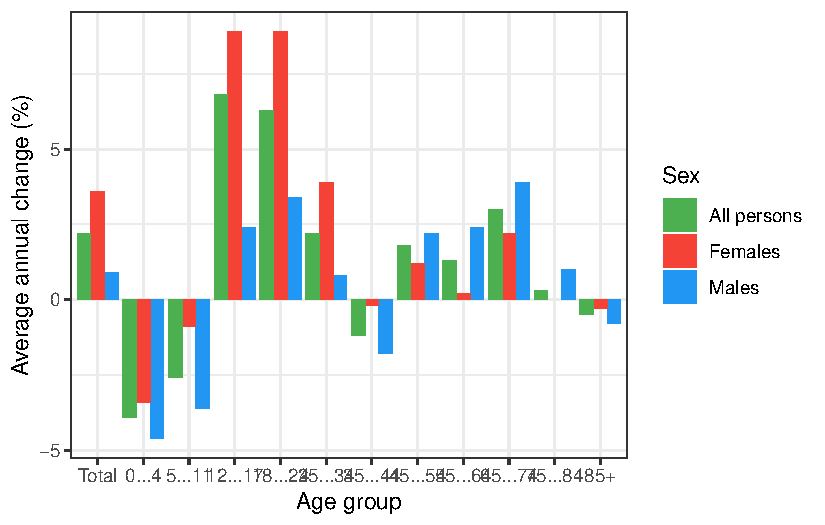
\includegraphics{./chap2-cmhc_files/figure-pdf/fig-cmhc-csa-1.pdf}

}

\end{figure}

\hypertarget{changes-over-time-by-age-aroup}{%
\subsection{Changes Over Time by Age
Aroup}\label{changes-over-time-by-age-aroup}}

\hypertarget{male-patients}{%
\subsubsection{Male Patients}\label{male-patients}}

\begin{figure}

\caption{\label{fig-cmhc-cam}Male Contact Rate Trends by Age Group,
2005-2020}

{\centering 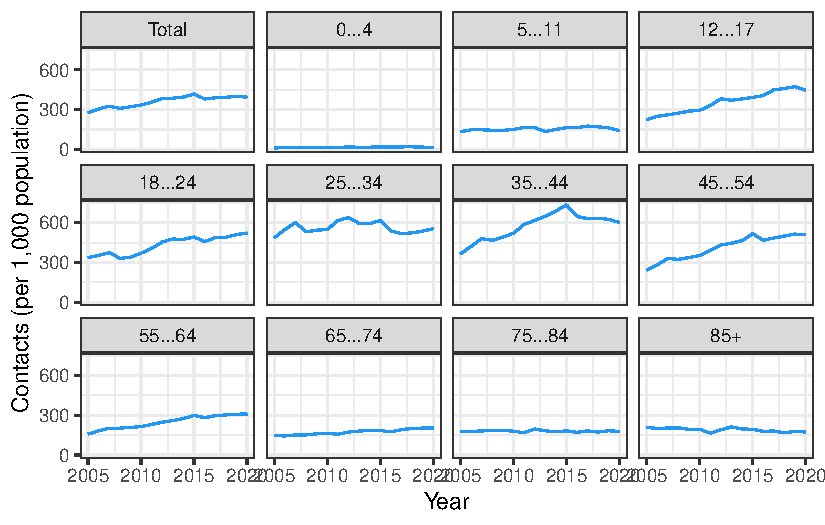
\includegraphics{./chap2-cmhc_files/figure-pdf/fig-cmhc-cam-1.pdf}

}

\end{figure}

\hypertarget{female-patients}{%
\subsubsection{Female Patients}\label{female-patients}}

\begin{figure}

\caption{\label{fig-cmhc-caf}Female Contact Rate Trends by Age Group,
2005-2020}

{\centering 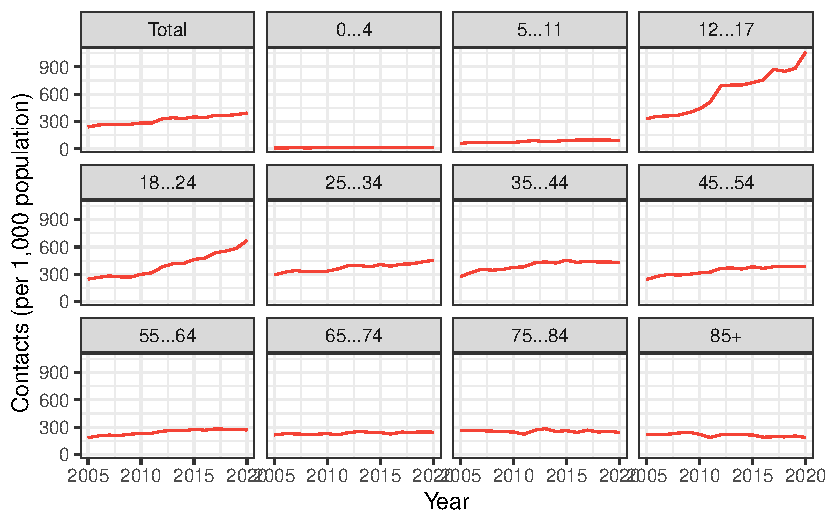
\includegraphics{./chap2-cmhc_files/figure-pdf/fig-cmhc-caf-1.pdf}

}

\end{figure}

\hypertarget{summary-4}{%
\subsection{Summary}\label{summary-4}}

5-year change over 2016-2020:

\begin{itemize}
\item
  Contacts rate for children aged 0-11 significantly declined for both
  sex.
\item
  A notable increase in contacts among young individuals aged 12-24,
  with females showing a particularly strong uptick.
\item
  Middle-aged and elderly individuals (45-74) showed an upward trend in
  contacts rate, with males contributing significantly to this increase.
\end{itemize}

15-year change over 2005-2020:

\begin{itemize}
\item
  Between 2005 and 2020, there was a modest increase in contact rates
  for both males and females.
\item
  Males aged 12-54 had the highest contact rates among all age groups,
  and it also shows an increasing trend in the 15 years.
\item
  Contact rates for young females (aged 12-24) roughly tripled during
  the 15 years, while rates for other age groups remained stable.
\end{itemize}

\bookmarksetup{startatroot}

\hypertarget{specialist-homelessness-services}{%
\chapter{Specialist Homelessness
Services}\label{specialist-homelessness-services}}

\hypertarget{about-the-data-2}{%
\section{About the Data}\label{about-the-data-2}}

This section is about the clients who identified as having a current
mental health issue and received specialist homelessness services (SHS).

\textbf{Specialist homelessness service(s) (SHS)} is assistance provided
by a specialist homelessness agency to a client aimed at responding to
or preventing homelessness. The specialist homelessness services in
scope for this collection include accommodation provision, assistance to
sustain housing, mental health services, family/relationship assistance,
disability services, drug/alcohol counselling, legal/financial services,
immigration/cultural services, domestic/family violence services, other
specialist services and general assistance and support.

The data used for this section came from
\href{https://www.aihw.gov.au/mental-health/topic-areas/specialist-homelessness-services}{Australian
Institute of Health and Welfare (AIHW)}.

\hypertarget{by-age-group-3}{%
\subsection{By Age Group}\label{by-age-group-3}}

\begin{figure}

\caption{\label{fig-shs-a}Recipients of SHS by Age Group, 2020-21}

{\centering 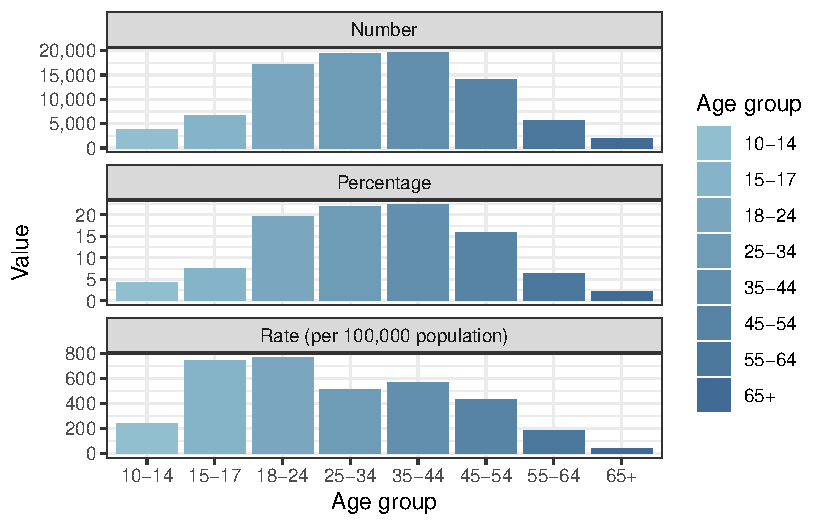
\includegraphics{./chap3-shs_files/figure-pdf/fig-shs-a-1.pdf}

}

\end{figure}

\hypertarget{by-sex-4}{%
\subsection{By Sex}\label{by-sex-4}}

\begin{figure}

\caption{\label{fig-shs-s}Recipients of SHS by Sex, 2020-21}

{\centering 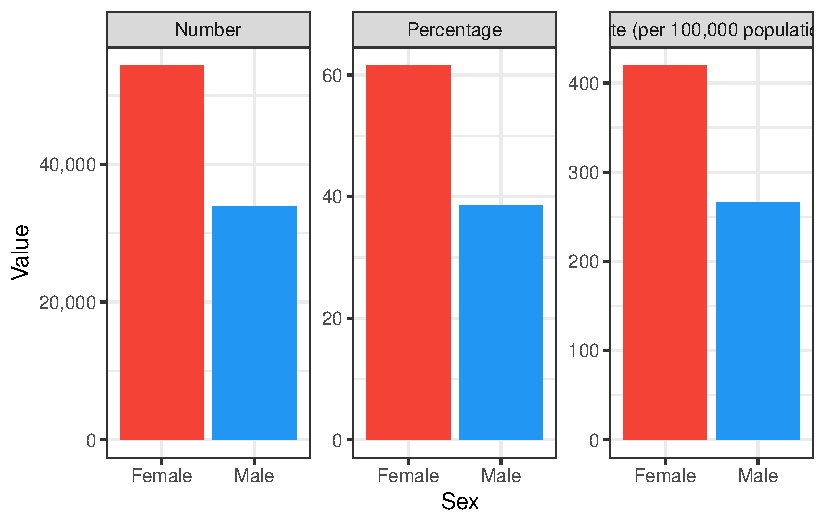
\includegraphics{./chap3-shs_files/figure-pdf/fig-shs-s-1.pdf}

}

\end{figure}

\hypertarget{summary-5}{%
\subsection{Summary}\label{summary-5}}

SHS recipients' rate:

\begin{itemize}
\item
  Young adults aged 15-24 constitute the highest percentage of those
  with current mental health issues who also receive SHS.
\item
  A decline in SHS recipient rates is observed as age increases.
\item
  Females significantly outnumber males in receiving these services.
\end{itemize}

SHS recipients' characteristics:

\begin{itemize}
\item
  The characteristics are similar to those of the general population -
  age distribution is bell-shaped and 25-44.
\item
  The number and percentage of female recipients are much higher than
  males.
\end{itemize}

\bookmarksetup{startatroot}

\hypertarget{residential-mental-health-care-rmhc-services}{%
\chapter{Residential Mental Health Care (RMHC)
Services}\label{residential-mental-health-care-rmhc-services}}

\hypertarget{about-the-data-3}{%
\section{About the Data}\label{about-the-data-3}}

\textbf{Residential mental health care (RMHC)} services provide
specialised mental health care on an overnight basis in a domestic-like
environment. RMHC services may include rehabilitation, treatment or
extended care.

The data used for this section came from
\href{https://www.aihw.gov.au/mental-health/topic-areas/residential-services}{Australian
Institute of Health and Welfare (AIHW)}.

\hypertarget{resident-characteristics}{%
\section{Resident Characteristics}\label{resident-characteristics}}

\emph{Note: A \textbf{resident} is a person who receives residential
care intended to be for a minimum of 1 night.}

\hypertarget{by-age-group-4}{%
\subsection{By Age Group}\label{by-age-group-4}}

\begin{figure}

\caption{\label{fig-rmhc-ra}People Accessing RMHC Services by Age Group,
2020-21}

{\centering 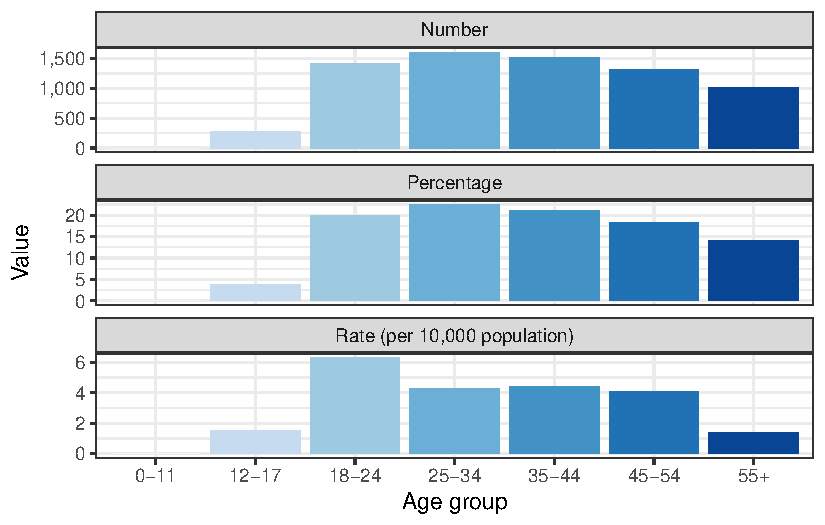
\includegraphics{./chap4-rmhc_files/figure-pdf/fig-rmhc-ra-1.pdf}

}

\end{figure}

\hypertarget{by-sex-5}{%
\subsection{By Sex}\label{by-sex-5}}

\begin{figure}

\caption{\label{fig-rmhc-rs}People Accessing RMHC Services by Sex,
2020-21}

{\centering 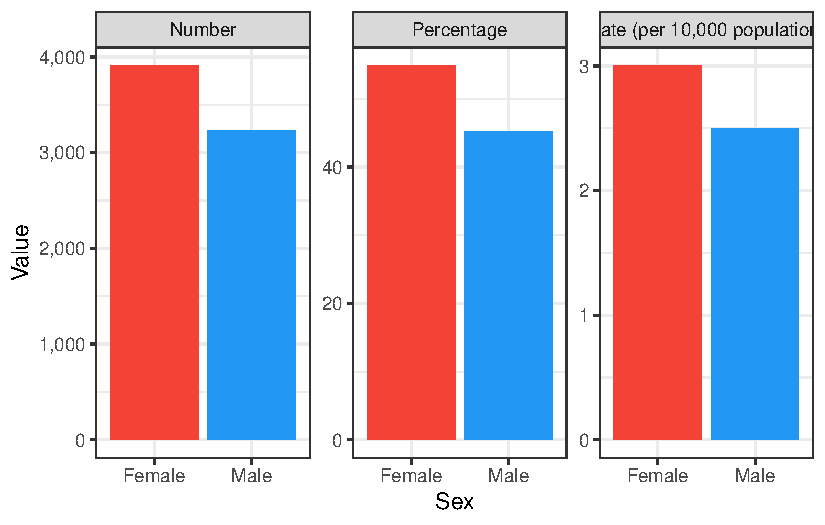
\includegraphics{./chap4-rmhc_files/figure-pdf/fig-rmhc-rs-1.pdf}

}

\end{figure}

\hypertarget{summary-6}{%
\subsection{Summary}\label{summary-6}}

\begin{itemize}
\item
  Individuals aged 18-24 have the highest rate of accessing RMHC, at
  approximately 6 per 10,000 population. For those aged 25-54, the rate
  stabilizes at around 4 per 10,000.
\item
  Females have a higher rate, population, and percentage of accessing
  RMHC.
\end{itemize}

\hypertarget{rmhc-service-episodes-rate}{%
\section{RMHC Service Episodes Rate}\label{rmhc-service-episodes-rate}}

\textbf{Episodes of residential care} are defined as a period of care
between the start of residential care (either through the formal start
of the residential stay or the start of a new reference period (that is,
1 July)) and the end of residential care (either through the formal end
of residential care, commencement of leave intended to be greater than 7
days, or the end of the reference period (that is, 30 June)). An
individual can have one or more episodes of care during the reference
period.

\hypertarget{general-sex-and-age-characteristics}{%
\subsection{General Sex and Age
Characteristics}\label{general-sex-and-age-characteristics}}

\hypertarget{by-sex-and-age-group}{%
\subsubsection{By Sex and Age Group}\label{by-sex-and-age-group}}

\begin{figure}

\caption{\label{fig-rmhc-gsa}Episodes Rate by Age Group and Sex,
2020-21}

{\centering 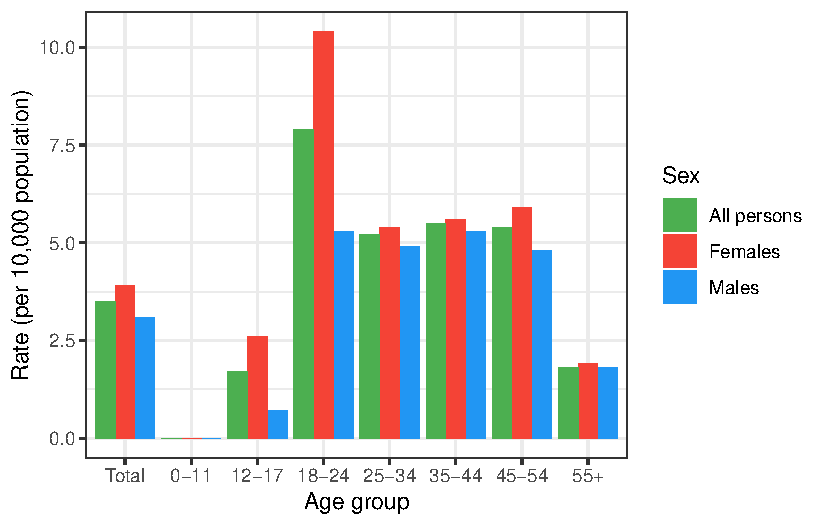
\includegraphics{./chap4-rmhc_files/figure-pdf/fig-rmhc-gsa-1.pdf}

}

\end{figure}

\hypertarget{summary-7}{%
\subsubsection{Summary}\label{summary-7}}

\begin{itemize}
\item
  Females aged 18-24 exhibit an exceptionally high episode rate,
  exceeding 10 per 10,000 population.
\item
  For ages 25-54, the episode rates are generally similar across both
  genders, though slightly higher for females, with an average of about
  5 per 10,000 population.
\item
  Young girls aged 12-17 experience exceptionally higher episode rates
  than boys in the same age group.
\end{itemize}

\hypertarget{sex-and-age-characteristics-by-states-or-territories}{%
\subsection{Sex and Age Characteristics by States or
Territories}\label{sex-and-age-characteristics-by-states-or-territories}}

\hypertarget{by-sex-and-states-or-territories-1}{%
\subsubsection{By Sex and States or
Territories}\label{by-sex-and-states-or-territories-1}}

\begin{figure}

\caption{\label{fig-rmhc-gss}Episodes Rate by Sex and States or
Territories, 2020-21}

{\centering 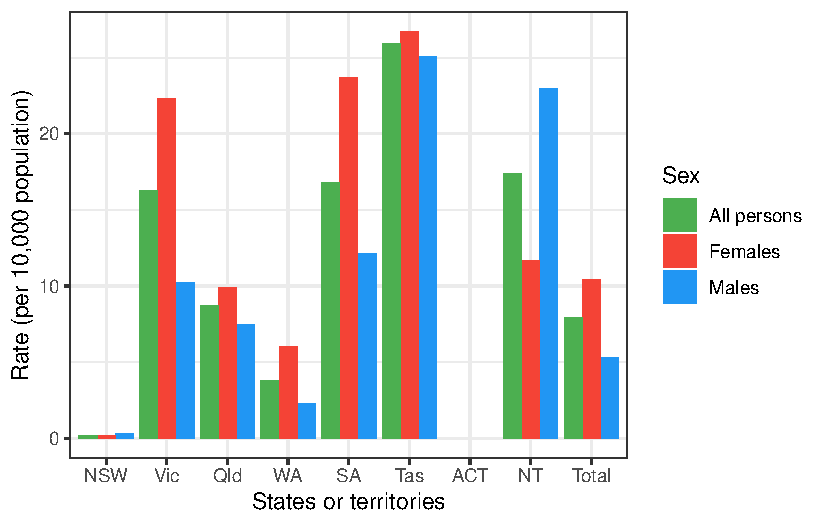
\includegraphics{./chap4-rmhc_files/figure-pdf/fig-rmhc-gss-1.pdf}

}

\end{figure}

\emph{Note: Data for \textbf{ACT} is not applicable and should not be
interpreted as zero. Some data for \textbf{NSW} is rounded to zero.}

\hypertarget{by-sex-age-group-states-or-territories}{%
\subsubsection{By Sex, Age Group, States or
Territories}\label{by-sex-age-group-states-or-territories}}

\begin{figure}

\caption{\label{fig-rmhc-gsas}Episodes Rate by Sex, Age Group, States or
Territories, 2020-21}

{\centering 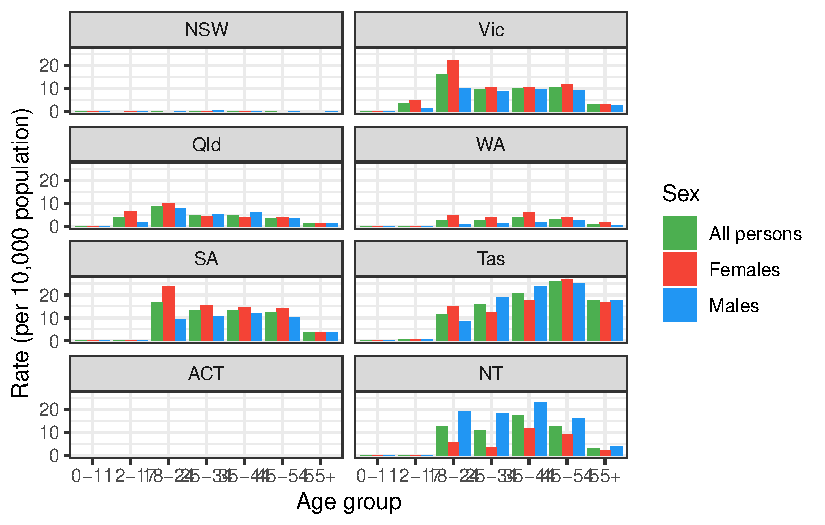
\includegraphics{./chap4-rmhc_files/figure-pdf/fig-rmhc-gsas-1.pdf}

}

\end{figure}

\emph{Note: Data for \textbf{ACT} is not applicable and should not be
interpreted as zero. Some data for \textbf{NSW} is rounded to zero.}

\hypertarget{summary-8}{%
\subsubsection{Summary}\label{summary-8}}

\begin{itemize}
\item
  Tasmania has the highest episode rate among all states or territories,
  while New South Wales registers have the lowest, nearly reaching zero.
\item
  Female rates are generally higher across most states or territories,
  notably among young women aged 18-24 in Victoria and South Australia.
\item
  The Northern Territory is an exception where the male rate is about
  double the female rate, attributed to a low female rate.
\item
  Episode rates in Queensland and Western Australia are moderate, with
  all values less than 10 per 10,000 population.
\end{itemize}

\hypertarget{episode-rates-changes-over-time}{%
\subsection{Episode Rates Changes Over
Time}\label{episode-rates-changes-over-time}}

\hypertarget{average-annual-episodes-change}{%
\subsubsection{Average Annual Episodes
Change}\label{average-annual-episodes-change}}

\begin{figure}

\caption{\label{fig-rmhc-asa}Average Annual Episodes Change by Sex and
Age group, 2016--17 to 2020--21}

{\centering 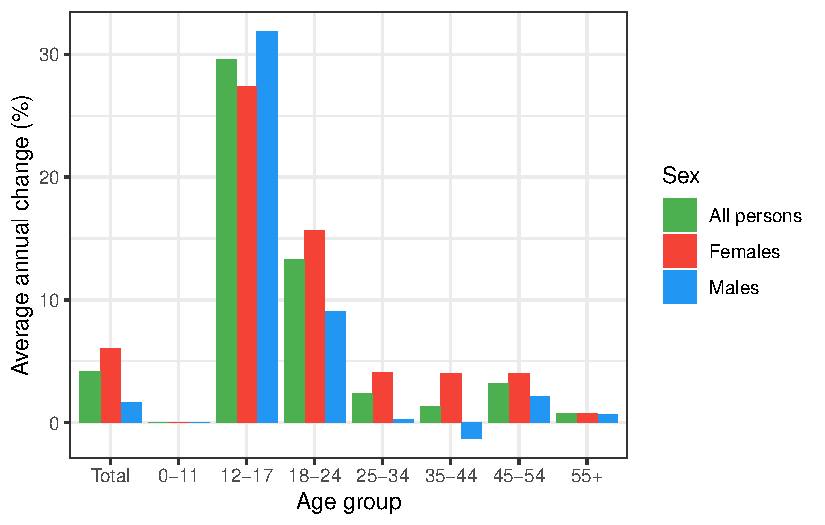
\includegraphics{./chap4-rmhc_files/figure-pdf/fig-rmhc-asa-1.pdf}

}

\end{figure}

\hypertarget{episodes-changes-over-the-year-by-age-and-sex}{%
\subsubsection{Episodes Changes Over the Year by Age and
Sex}\label{episodes-changes-over-the-year-by-age-and-sex}}

\begin{figure}

\caption{\label{fig-rmhc-cras}Change of Episodes Rate by Sex Over Year
2005--06 to 2020--21}

{\centering 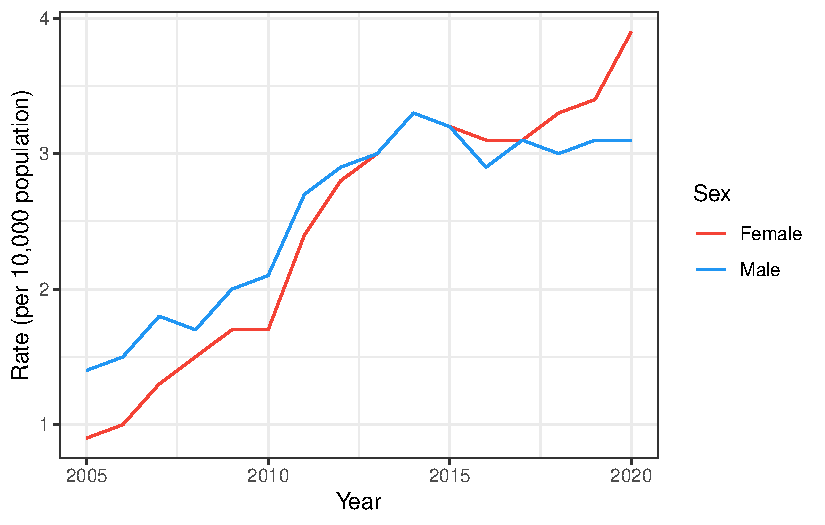
\includegraphics{./chap4-rmhc_files/figure-pdf/fig-rmhc-cras-1.pdf}

}

\end{figure}

\begin{figure}

\caption{\label{fig-rmhc-cnas}Change of Episodes Number by Age and Sex
Over Year 2005--06 to 2020--21}

{\centering 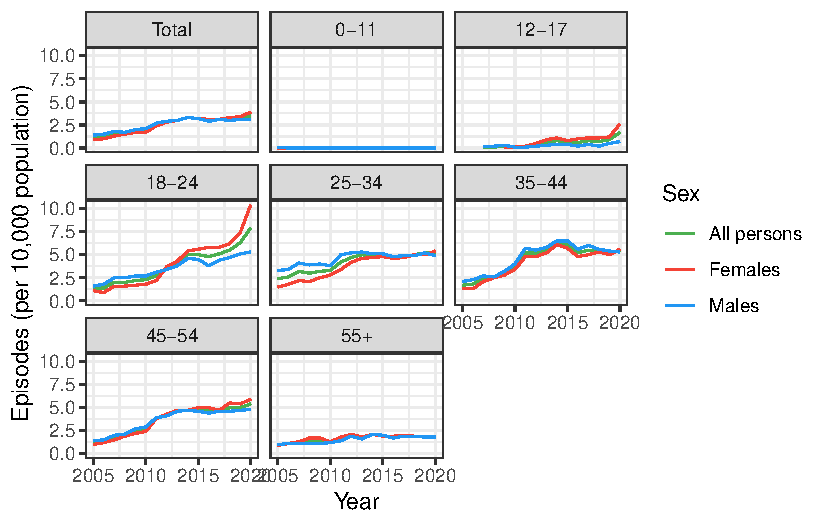
\includegraphics{./chap4-rmhc_files/figure-pdf/fig-rmhc-cnas-1.pdf}

}

\end{figure}

\hypertarget{summary-9}{%
\subsection{Summary}\label{summary-9}}

\begin{itemize}
\item
  From 2005-06 to 2020-21, the female episode rate quadrupled from 0.9
  to 3.9, while the male rate doubled.
\item
  From 2005 to 2012, the male episode rate was higher than females;
  between 2012 and 2015, the rates for both genders were the same; from
  2015 onwards, the female episode rate surpassed the male rate. This
  symptom is largely driven by the trend in young women aged 18-24.
\end{itemize}

\bookmarksetup{startatroot}

\hypertarget{psychosocial-disability-support-services}{%
\chapter{Psychosocial Disability Support
Services}\label{psychosocial-disability-support-services}}

\textbf{Psychosocial disability* support services} are critical in
assisting people with psychosocial disability overcome functional
limitations (for example, with communication, daily living or self-care)
and facilitating full and equal participation in the community.

This section presents information on specialist disability support
services provided under the National Disability Insurance Scheme (NDIS)
to participants with a \textbf{primary disability*} of psychosocial
disability.

The data used for this section came from
\href{https://www.aihw.gov.au/mental-health/topic-areas/psychosocial-disability-support}{Australian
Institute of Health and Welfare (AIHW)}.

\hypertarget{by-states-or-territory}{%
\section{By States or Territory}\label{by-states-or-territory}}

\begin{figure}

\caption{\label{fig-dis-s}NDIS Psychosocial Participants, by States or
Territory, as of Dec 2021}

{\centering 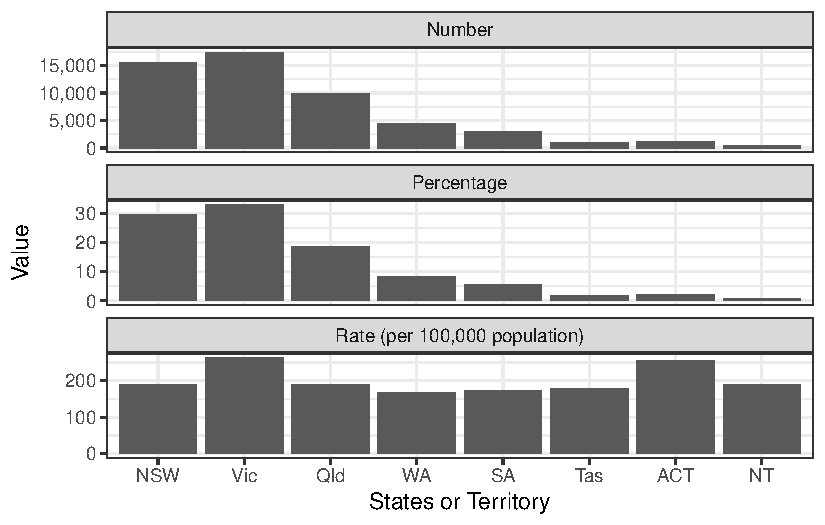
\includegraphics{./chap5-dis_files/figure-pdf/fig-dis-s-1.pdf}

}

\end{figure}

\hypertarget{by-age}{%
\section{By Age}\label{by-age}}

\begin{figure}

\caption{\label{fig-dis-a}NDIS Psychosocial Participants, by Age Group,
as of Dec 2021}

{\centering 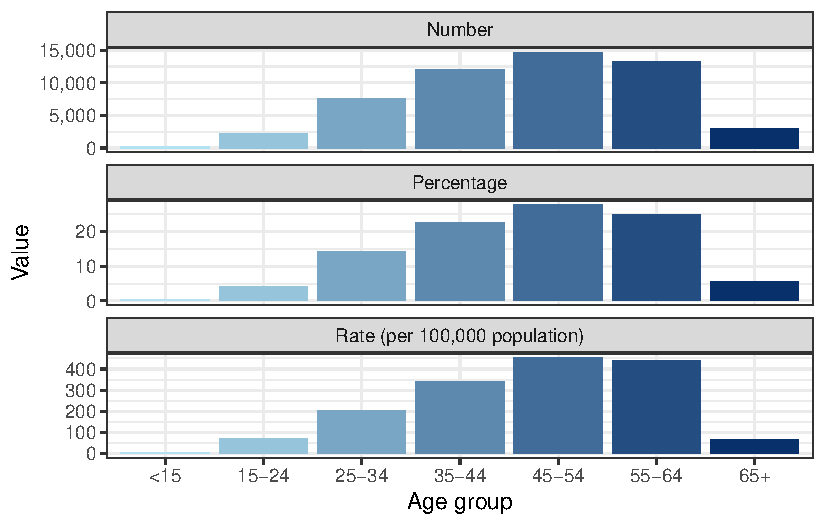
\includegraphics{./chap5-dis_files/figure-pdf/fig-dis-a-1.pdf}

}

\end{figure}

\hypertarget{summary-10}{%
\section{Summary}\label{summary-10}}

\begin{itemize}
\item
  Vic and ACT have the highest rates, with approximately 250 per
  100,000. Other states and territories show similar, lower rates,
  ranging from 170 to 190 per 100,000.
\item
  The rate, number, and percentage of active patients all display a
  similar trend across age groups, increasing progressively with age but
  experiencing a decline after age 65+.
\end{itemize}



\end{document}
